%% LyX 2.3.6.2 created this file.  For more info, see http://www.lyx.org/.
%% Do not edit unless you really know what you are doing.
\documentclass{article}
\usepackage{lmodern}
\usepackage{lmodern}
\usepackage[T1]{fontenc}
\usepackage[utf8]{inputenc}
\setcounter{secnumdepth}{-1}
\usepackage{amsmath}
\usepackage{amssymb}
\usepackage{graphicx}
\PassOptionsToPackage{normalem}{ulem}
\usepackage{ulem}
\usepackage{subscript}
\usepackage[unicode=true,
 bookmarks=false,
 breaklinks=false,pdfborder={0 0 1},backref=section,colorlinks=false]
 {hyperref}
\hypersetup{
 hidelinks,pdfcreator={LaTeX via pandoc}}

\makeatletter
\@ifundefined{date}{}{\date{}}
%%%%%%%%%%%%%%%%%%%%%%%%%%%%%% User specified LaTeX commands.
% Options for packages loaded elsewhere


%
\usepackage{iftex}
\ifPDFTeX
  \usepackage{textcomp}% provide euro and other symbols
\else % if luatex or xetex
  \usepackage{unicode-math}
\defaultfontfeatures{Scale=MatchLowercase}
  \defaultfontfeatures[\rmfamily]{Ligatures=TeX,Scale=1}
\fi
% Use upquote if available, for straight quotes in verbatim environments
\IfFileExists{upquote.sty}{\usepackage{upquote}}{}
\IfFileExists{microtype.sty}{% use microtype if available
  \usepackage[]{microtype}
  \UseMicrotypeSet[protrusion]{basicmath} % disable protrusion for tt fonts
}{}

\@ifundefined{KOMAClassName}{% if non-KOMA class
  \IfFileExists{parskip.sty}{%
    \usepackage{parskip}
  }{% else
    \setlength{\parindent}{0pt}
    \setlength{\parskip}{6pt plus 2pt minus 1pt}}
}{% if KOMA class
  \KOMAoptions{parskip=half}}

\usepackage{xcolor}
\IfFileExists{xurl.sty}{\usepackage{xurl}}{} % add URL line breaks if available
\IfFileExists{bookmark.sty}{\usepackage{bookmark}}{\usepackage{hyperref}}

\urlstyle{same} % disable monospaced font for URLs

\def\maxwidth{\ifdim\Gin@nat@width>\linewidth\linewidth\else\Gin@nat@width\fi}
\def\maxheight{\ifdim\Gin@nat@height>\textheight\textheight\else\Gin@nat@height\fi}

% Scale images if necessary, so that they will not overflow the page
% margins by default, and it is still possible to overwrite the defaults
% using explicit options in \includegraphics[width, height, ...]{}
\setkeys{Gin}{width=\maxwidth,height=\maxheight,keepaspectratio}
% Set default figure placement to htbp

\def\fps@figure{htbp}

\setlength{\emergencystretch}{3em} % prevent overfull lines
\providecommand{\tightlist}{%
  \setlength{\itemsep}{0pt}\setlength{\parskip}{0pt}}
 % remove section numbering
\ifLuaTeX
  \usepackage{selnolig}% disable illegal ligatures
\fi

\title{Exams (without answers) of module

Transient Groundwater Flow

from 2006 onwards}
\author{}

\makeatother

\begin{document}
\title{UNESCO-IHE}
\title{Exams Transient Groundwater FLow - from 2006-2022}
\author{Prof.dr.ir.T.N.Olsthoorn}
\date{\emph{\today}}

\maketitle
\tableofcontents{}

\section*{Open-book exam (1h), Feb 7, 2022}

\subsection*{Question 1:}

A well is installed at 250 m distance from a river. The well fully
penetrates the aquifer. The aquifer is unconfined, it has a conductivity
of k= 30~m/d and a representative thickness of 40~m, which may be
assumed constant. It further has a storage coefficient (specific yield)
of S=0.20. The well extracts water at a rate of \emph{Q}=1200~m\textsuperscript{3}/d
during exactly 7~days, after which it stops. The questions refer
to the drawdown in point p at 50 m from the well on the line through
the well perpendicular to the river as shown in the figure.

\begin{figure}
\begin{centering}
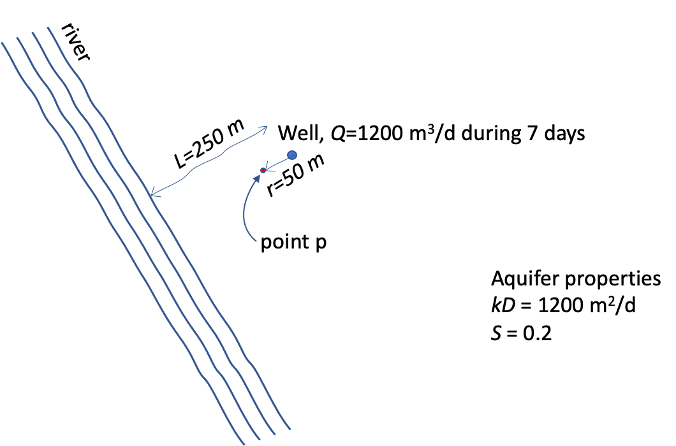
\includegraphics[width=0.8\textwidth]{pictures/2022_1}
\par\end{centering}
\caption{Well adjacent to a straight fully penetrating river. The aquifer is
homogeneous and extends to infinity.This is clearly a well in an aquifer
with constant transmissivity, for which the well-known Theis solution
is applicable. To obtain values for the Theis well function, you can
make use of the Theis type curve shown below.}

\end{figure}

\begin{figure}
\begin{centering}
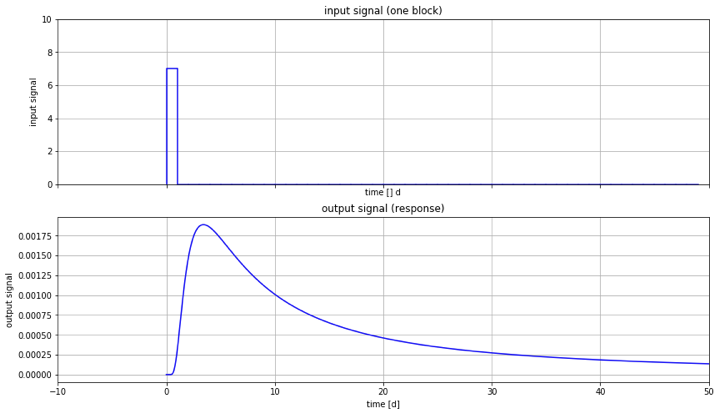
\includegraphics[width=0.8\textwidth]{pictures/2022_2}
\par\end{centering}
\caption{Theis type curve, i.e., the Theis well function as a function of $1/u$}

\end{figure}

\begin{enumerate}
\item What will be the drawdown at point \emph{p} at $t=7$ d after the
start of the extraction? 
\item What will be the drawdown at point p 14 days after the start of the
extraction, i.e., 7 days after the well has started pumping? 
\end{enumerate}

\subsection*{Question 2:}

The picture shows an aquifer bounded by a fully penetrating river
at \emph{x=0}. The aquifer is unbounded to the right and has a transmissivity
and a specific yield as indicated in the picture. Note that the transmissivity
may be considered constant. The river water level varies continuously
according to a sinewave with a cycle time of \emph{T= 1} d and an
amplitude of \emph{A=1.2} m.

\begin{figure}
\begin{centering}
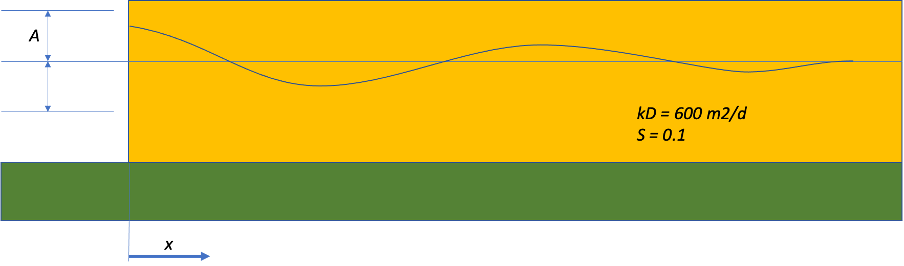
\includegraphics[width=0.8\textwidth]{pictures/2022_3}
\par\end{centering}
\caption{Aquifer bounded by fully penetrating water body with fluctuating water
level at x=0. The aquifer extents at the right to infinity. Shown
is the water table (or head) at an arbitrary time.}

\end{figure}

\begin{enumerate}
\item What is the maximum and minimum head at \emph{x = 25} m and at \emph{x
= 100} m? 
\item What is the delay of the wave at \emph{x = 100} m relative to the
wave at \emph{x = 0} m? 
\item By how much (i.e., by how large a factor) does this delay change if
the storage coefficient would be 100 times as small as the given value,
i.e., if it would be $S=0.001$ instead of $S=0.1$? 
\end{enumerate}
The picture below shows an aquifer of limited lateral extent. To the
left, at \emph{x = 0}, it is bounded by a fully penetrating surface
water body, such as a lake. To the right, at \emph{x = L}, it is bounded
by an impervious land mass as shown. The aquifer properties are shown
in the picture, but you don't need them to answer the questions. The
water level of the lake and the groundwater table are initially flat
at a level equal to \emph{h=0}~m as indicated by the horizontal blue
line. At $t\ =\ 0$, the water level of the lake suddenly changes
upward by an amount \emph{A} as indicated. Ignore other hydrological
features like rain and evapotranspiration. Only the effect of the
sudden change of the lake level is considered.

\begin{figure}
\begin{centering}
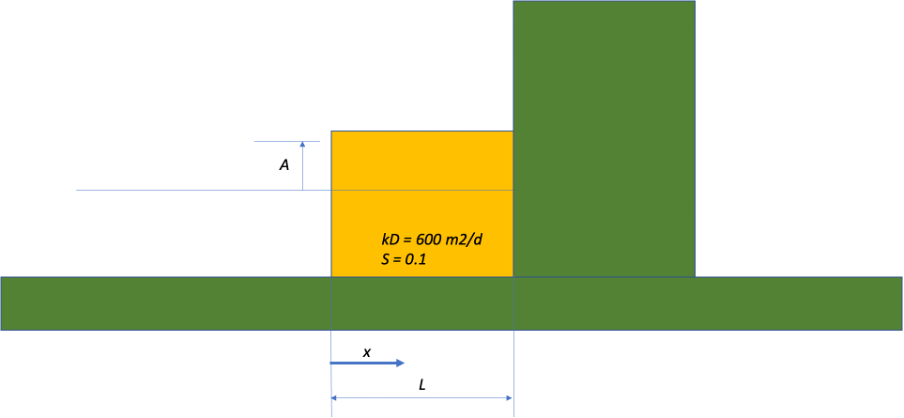
\includegraphics[width=0.8\textwidth]{pictures/2022_4}
\par\end{centering}
\caption{Picture of the aquifer with fully penetrating water body at $x=0$
and impervious mass at $x=L$}

\end{figure}

\begin{enumerate}
\item What are the boundary conditions at \emph{x=0} and \emph{x=L}? 
\item Describe how the head in the aquifer will develop over time due to
the sudden change at \emph{x=0} and \emph{t=0}. Your description must
include the situation at $t=0$ and at $t=\infty$. 
\end{enumerate}

\section*{Closed-book exam (1h), Feb 23, 2021}

\subsection*{Question 1:}
\begin{enumerate}
\item When pumping from a confined aquifer, all extracted water comes from
storage. But what is the precise physical mechanism that causes the
release of water from this type of aquifer? Explain. 
\item What is the so-called air-entry pressure and how does it relate to
the capillary fringe? Explain. 
\item A confined aquifer system has a loading efficiency of LE = 0.6. If
the barometer pressure increases with the equivalent of 40 cm water
column, by how much does the pressure in the aquifer change? By how
much does the head (water level in a piezometer in this aquifer) change?
Explain and show. 
\item What is the difference between a Theis and a Hantush situation? The
answer must contain the difference between the two situations as and
what the physical origin is of the water pumped from a well in both
these situations. 
\end{enumerate}

\subsection*{Question 2:}

The solution for the head in a confined aquifer driven by surface
water that varies according to a sine at x=0 is given by

\[
h_{x,t}=Ae^{-ax}\sin\left(\omega t-ax\right)\text{, with }a=\sqrt{\frac{\omega S}{2kD}}
\]

\begin{enumerate}
\item Explain what the parameters are with their dimension.
\item What is the velocity of the wave in the subsurface? Explain mathematically. 
\item What are the so-called envelopes? Explain and show them mathematically. 
\end{enumerate}

\subsection*{Question 3:}

The dynamic change of head in a strip of land of limited width like
the one that is shown below can be computed using the simple formula
for a half-infinite aquifer, but then we must apply superposition
using so-called mirror ditches. In the figure below the water level
at the left-hand side has just jumped up by \emph{A} m and that at
the right-and side by \emph{B} m. The head for t=0.29 d is shown.
The lower picture shows the applied mirror/superposition scheme.
\begin{enumerate}
\item Is the shown mirror/superposition scheme used for the superposition
correct? Clearly motivate your answer, a simple yes or no is not accepted. 
\end{enumerate}
\begin{figure}
\begin{centering}
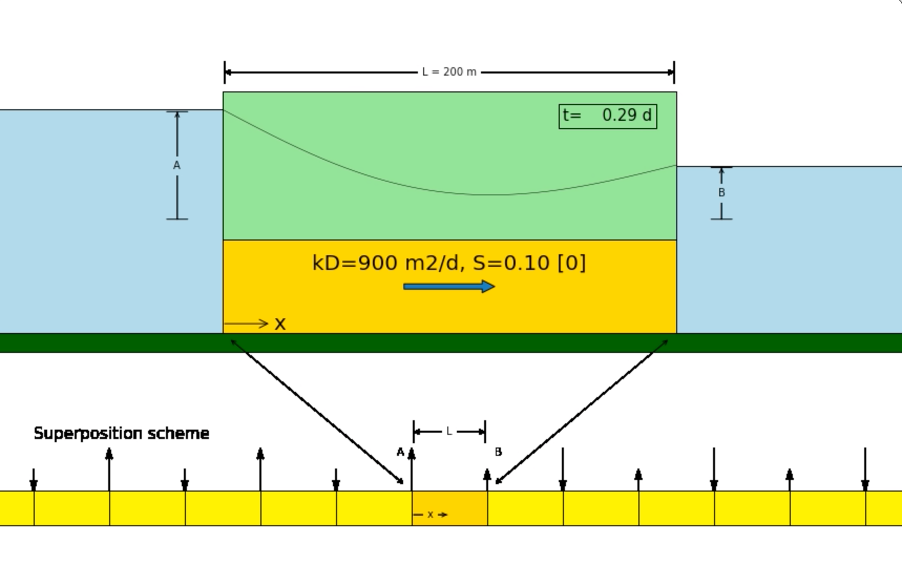
\includegraphics[width=0.8\textwidth]{pictures/2021_1}
\par\end{centering}
\caption{Strip of land bounded by fully penetrating surface water (top) and
superposition scheme (bottom).}

\end{figure}


\subsection*{Question 4:}

During a pumping test with an extraction of $Q=650\,\mathrm{m^{3}/d}$,
the drawdown is measured in an observation well at $r=50\,\mathrm{m}$
distance from the well, sufficient to ignore any influence of partial
penetration on the measurements. The measured drawdown in this piezometer
is shown graphically versus the log of time in days.

\begin{figure}
\begin{centering}
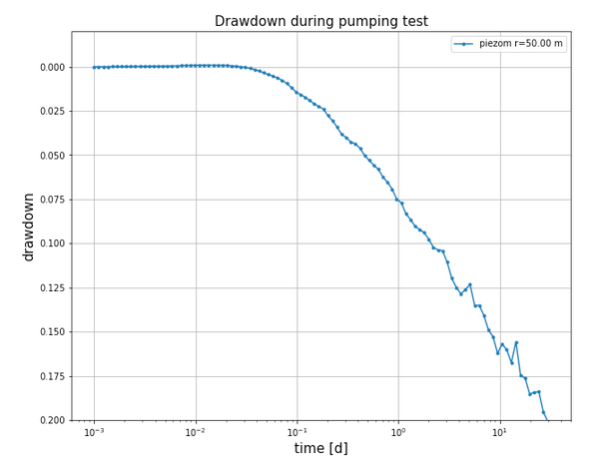
\includegraphics[width=0.8\textwidth]{pictures/2021_2}
\par\end{centering}
\caption{Measured drawdown during pumping test.}

\end{figure}

The formula for the drawdown that is expected to fit the data for
sufficiently large times is

\[
s_{r,t}\,=\,\frac{Q}{4\pi kD}\ln\left(\frac{2.25kDt}{r^{2}S}\right)
\]

\begin{enumerate}
\item Do these data represent a Theis (confined/unconfined) or a Hantush
(semi-confined) situation? Motivate your answer (a single yes or no
is not accepted). 
\item Determine the transmissivity of the aquifer 
\item Determine the storage coefficient of the aquifer 
\item What will be the radius of influence of this pumping test for $t=5$
days? 
\end{enumerate}

\section{Closed book exam (1h), Feb 4, 2020}

\subsection{Question 1:}
\begin{enumerate}
\item Explain what is meant by air-entry pressure, and how you interpret
it in terms of groundwater? 
\item What happens to the water level in a piezometer installed in a confined
aquifer if suddenly a load equivalent to a pressure increase $\Delta p$
is placed on ground surface? 
\item What happens to the water level in a piezometer if the barometer pressure
suddenly change by an amount $\Delta p$? 
\item Explain what causes the difference between the answers to questions
2. And 3. 
\item If a pressure transducer is fixed in a piezometer, below the water
level at a given elevation, then what changes would it register in
the two situations described in questions 2 and 3? (A pressure transducer
measures and registers the absolute pressure, i.e. water + air). 
\end{enumerate}

\subsection{Question 2:}

Let the time-dependent change of head in a strip of land with width
\emph{\ensuremath{L}} {[}m{]} between two ditches be caused by a sudden
change of water level equal to \emph{\ensuremath{A}} {[}m{]} at the
left ditch and equal to \emph{\ensuremath{B}} {[}m{]} at the right
ditch. We know that this can be computed using the formula that is
valid for a half-infinite aquifer (that is an aquifer for which \emph{$x\ge0$})
bounded by surface water at $x=0$, if we apply superposition. The
formula for the half-infinite aquifer is

\[
s\left(x,t\right)=A\mathrm{erfc}\left(x\sqrt{\frac{S}{4kDt}}\right)
\]

In preparation of the superposition, a superposition scheme is drawn
(see figure below), which shows the strip of land in dark yellow and
the first few of the infinite series of mirror ditches. The arrows
indicate the direction and size of the change of head at each ditch.

\begin{figure}
\begin{centering}
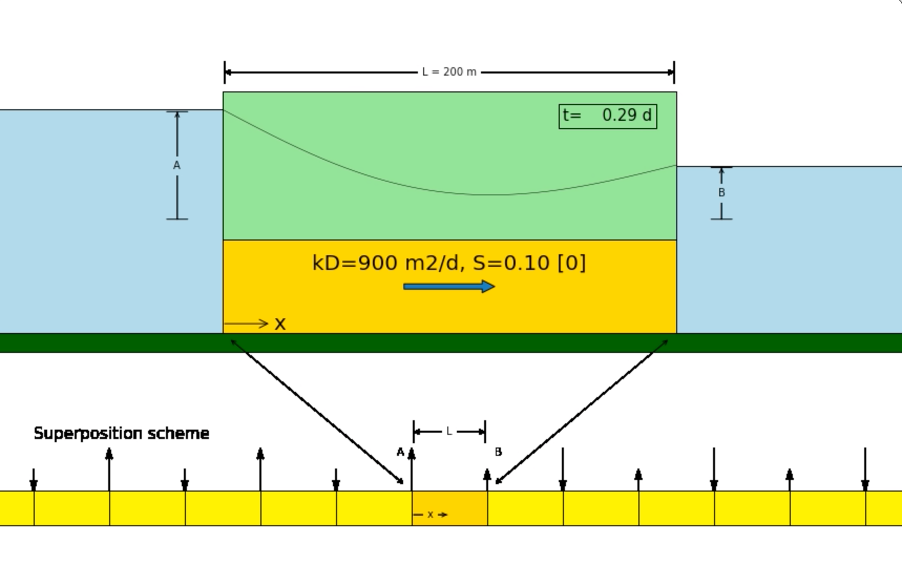
\includegraphics[width=0.8\textwidth]{pictures/2021_1}
\par\end{centering}
\caption{Strip of land bounded by fully penetrating surface water (top) and
superposition scheme (bottom).}

\end{figure}

\begin{enumerate}
\item Is this scheme correct? Explain why or why not that is the case. 
\end{enumerate}

\subsection{Question 3:}

The first term of formula describing the drainage of a strip of land
of with $L=2b$, the head at $t=0$ is uniform and equal to \emph{$A$}
{[}m{]} above the ditches on either side, is given by

\[
s\left(x,t\right)=A\frac{4}{\pi}\cos\left(\frac{\pi x}{2b}\right)\exp\left(-\left(\frac{\pi}{2}\right)^{2}\frac{t}{T}\right)
\]

with

\[
T=\frac{b^{2}S}{kD}
\]

\begin{enumerate}
\item What does this equation tell you? What's happening here? What name
would you give to \emph{T} ? Also explain why. 
\item What is the halftime of this drainage process? Explain, and show it
mathematically. 
\end{enumerate}

\subsection{Question 4:}

How would you compare the rate of drainage of a desert that is 500
km wide between surface -water boundaries and an arable field of 100
m wide between ditches, if both have the same aquifer properties?

\subsection{Question 5:}

The simplified Theis solution for the drawdown due to a pumping well
in a (un)confined aquifer reads

\[
s\left(r,t\right)=\frac{2.3Q}{4\pi kD}\log\left(\frac{2.25kDt}{r^{2}S}\right)
\]

A pumping test was carried out with an extraction of $Q=2400\,\mathrm{m^{3}/d}$.
The drawdown was measured in 3 observation wells.

The figure shows the measured drawdown $s$ in the observation wells
as a function of $t/r^{2}$ on logarithmic scale.

Answer the following questions
\begin{enumerate}
\item What is the transmissivity? Explain and compute it. 
\item What is the storage coefficient? Explain and compute it. 
\item If you had only the drawdown in the well itself instead of in observation
wells? What could you and what could you not determine, and why? 
\item What is the radius of influence? Explain and show it mathematically. 
\end{enumerate}
\begin{figure}
\begin{centering}
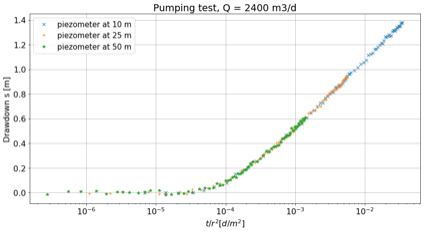
\includegraphics[width=0.8\textwidth]{pictures/2020_2}
\par\end{centering}
\caption{Measured drawdown of all piezometers versus $t/r^{2}$}

\end{figure}


\section{Closed book reexam (1h), March 2018}

\subsection{Question 1}
\begin{enumerate}
\item Explain what barometer efficiency (BE) is and how it physically works.
\item Explain in words what the characteristic halftime of an aquifer system
says about the behavior of the system?
\item Consider the parameters $L$ (system width), $kD$ (transmissivity)
and $S_{y}$ (specific yield), for each of these three parameters,
does in increase make the characteristic time larger or smaller?
\item What is capillary rise and what has capillary rise to do with air-entry
pressure?
\item When we extract water from a well in an infinitely extended aquifer,
from where does all this extracted water come? Explain your answer.
\end{enumerate}

\subsection{Question 2}

Consider an aquifer in direct contact with the ocean. The tide of
the ocean has an amplitude of $A=1.0\:\mathrm{m}$ and the cycle time
is $T=0.5\,\mathrm{d}$ (one full tide in 12h). The aquifer is confined.
The aquifer has the following properties: transmissivity $kD=900\,\mathrm{m^{2}/d}$
and storage coefficient $S_{y}=0.002$. We are only interested in
the effect of the tide land-inwards. The effect of the tidal fluctuation
on the groundwater head land-inward, $s$, obeys the following expression:

\[
s=A\,e^{-ax}\cos\left(\omega t-ax\right)\mbox{, where }a=\sqrt{\frac{\omega S}{2kD}}\mbox{, with }\omega=\frac{2\pi}{T}
\]

Notice that the difference between the uppercase \emph{S} and lowercase
\emph{s}.
\begin{enumerate}
\item Explain the parameters in the expression and given their dimension
\item What is the amplitude of the groundwater head fluctuation at 750 m
from the ocean? Explain your answer in a few words and fist show it
mathematically.
\item What is the delay of the head wave at 750 m from to the ocean with
respect to the tide? Hint: compute the velocity of the tidal wave
in the aquifer and then the time until the peak of the wave starting
at the ocean reaches $x=750\,\mathrm{m}$. Explain in a few words
your approach and start with showing your answer mathematically.
\end{enumerate}

\subsection{Question 3}

Consider a well in an infinite water-table (phreatic) aquifer. Drawdowns
are small compared to the thickness of the aquifer, so that $kD=900\,\mathrm{m^{2}/d}$
may be considered constant. The specific yield, $S_{y}=0.15$, is
also constant. As there are no boundary conditions, the drawdown by
the well follows the Theis equation. An approximation of which is

\[
s=\frac{Q}{4\pi kD}\ln\left(\frac{2.25kDt}{r^{2}S}\right)
\]

\begin{enumerate}
\item Derive a mathematical expression for the so-called \uline{radius
of influence}, that is, the distance beyond which the drawdown can
be neglected at a given time $t$. Notice that $\ln\left(\cdots\right)=2.3\log\left(\cdots\right)$.
\item As you can see from the equation, the drawdown is (approximately)
a logarithmic function in time. Derive a mathematical expression of
the increase of the drawdown per log cycle of time, that is, between
time \emph{t} and time \emph{$10t$.}
\item The figure below shows an example of an actual drawdown measured at
a piezometer at $r=100$ m from the well extracting $Q=1200\,\mathrm{m^{3}/d}$.
Determine the transmissivity of the aquifer.
\end{enumerate}
4) Bonus question (extra points): Determine the storage coefficient.

\begin{figure}
\begin{centering}
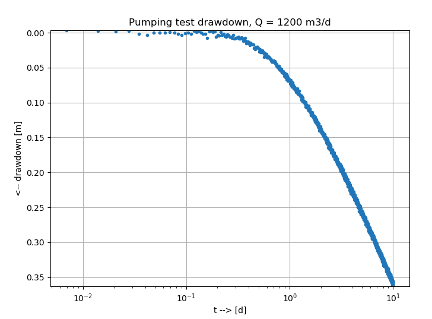
\includegraphics[width=0.8\textwidth]{pictures/2018_1}
\par\end{centering}
\caption{Measured drawdown in piezometer at \emph{$r=100\,\mathrm{m}$} from
well extracting $Q=1200\,\mathrm{m^{3}/d}$}

\end{figure}


\section{Closed book exam (1h), Feb 7, 2017}

\subsection{Question 1}
\begin{enumerate}
\item Someone says the barometer efficiency of the piezometer in his garden
is 25\%. What does that mean? Explain your answer telling how this
phenomenon physically works. 
\item A pressure logger that is installed in this piezometer measures absolute
pressure. What is absolute pressure? And what does this pressure gauge
see when the barometer rises by the equivalent of 40 cm of water column,
given the barometric efficiency of 25\%? 
\item What two properties determine the value of the specific (elastic)
storage coefficient? 
\item What does the air-entry value have to do with the thickness of the
capillary fringe/zone? Explain your answer. 
\end{enumerate}

\subsection{Question 2}

The transient drawdown of a well with a constant extraction \emph{Q}
in the case without any head boundary condition is mathematically
described by the Theis well drawdown:

\[
s=\frac{Q}{4\pi kD}W\left(\frac{r^{2}S}{4kDt}\right)
\]

that can be approximated by

\[
s\approx\frac{Q}{4\pi kD}\ln\left(\frac{2.25kDt}{r^{2}S}\right)
\]

\begin{enumerate}
\item Sketch both graphs such that s is on a linear scale (downward positive)
and time on a logarithmic horizontal scale. What's the difference
between the two? 
\item What is the drawdown per log-cycle of time, assuming that the approximation
is valid? 
\item What does "radius of influence" mean; how could you derive it from
the above approximation? 
\item Does the Theis drawdown reach a steady-state situation in the long
run? Explain your answer. 
\end{enumerate}
We know the total discharge (flow) across a ring at fixed distance
\emph{r} from the well in a confined aquifer is given by

\[
Q_{r,t}=Q_{0}e^{-u}\mbox{, with }u=\frac{r^{2}S}{4kDt}
\]

\begin{enumerate}
\item If you assume you are at a fixed distance $r$ from the well, could
you then formulate a characteristic time for the transient phenomenon
$Q(r,t)$ ? Explain your answer. 
\end{enumerate}
Below, we observe a hydrologist interpreting a transient pumping test
in a confined aquifer. He/she plotted the drawdown data on a double
log graph with drawdown \emph{$s$} vertically upward and $t/r^{2}$
horizontally. The data of this graph with the measurements was then
shifted over the Theis type-curve until the best possible match was
obtained. This match is shown in the figure. Given that the extraction
during the pumping test was 1200 m$^{3}$/d.
\begin{enumerate}
\item Determine the transmissivity $kD$ and the storage coefficient $S$. 
\end{enumerate}
\begin{figure}
\begin{centering}
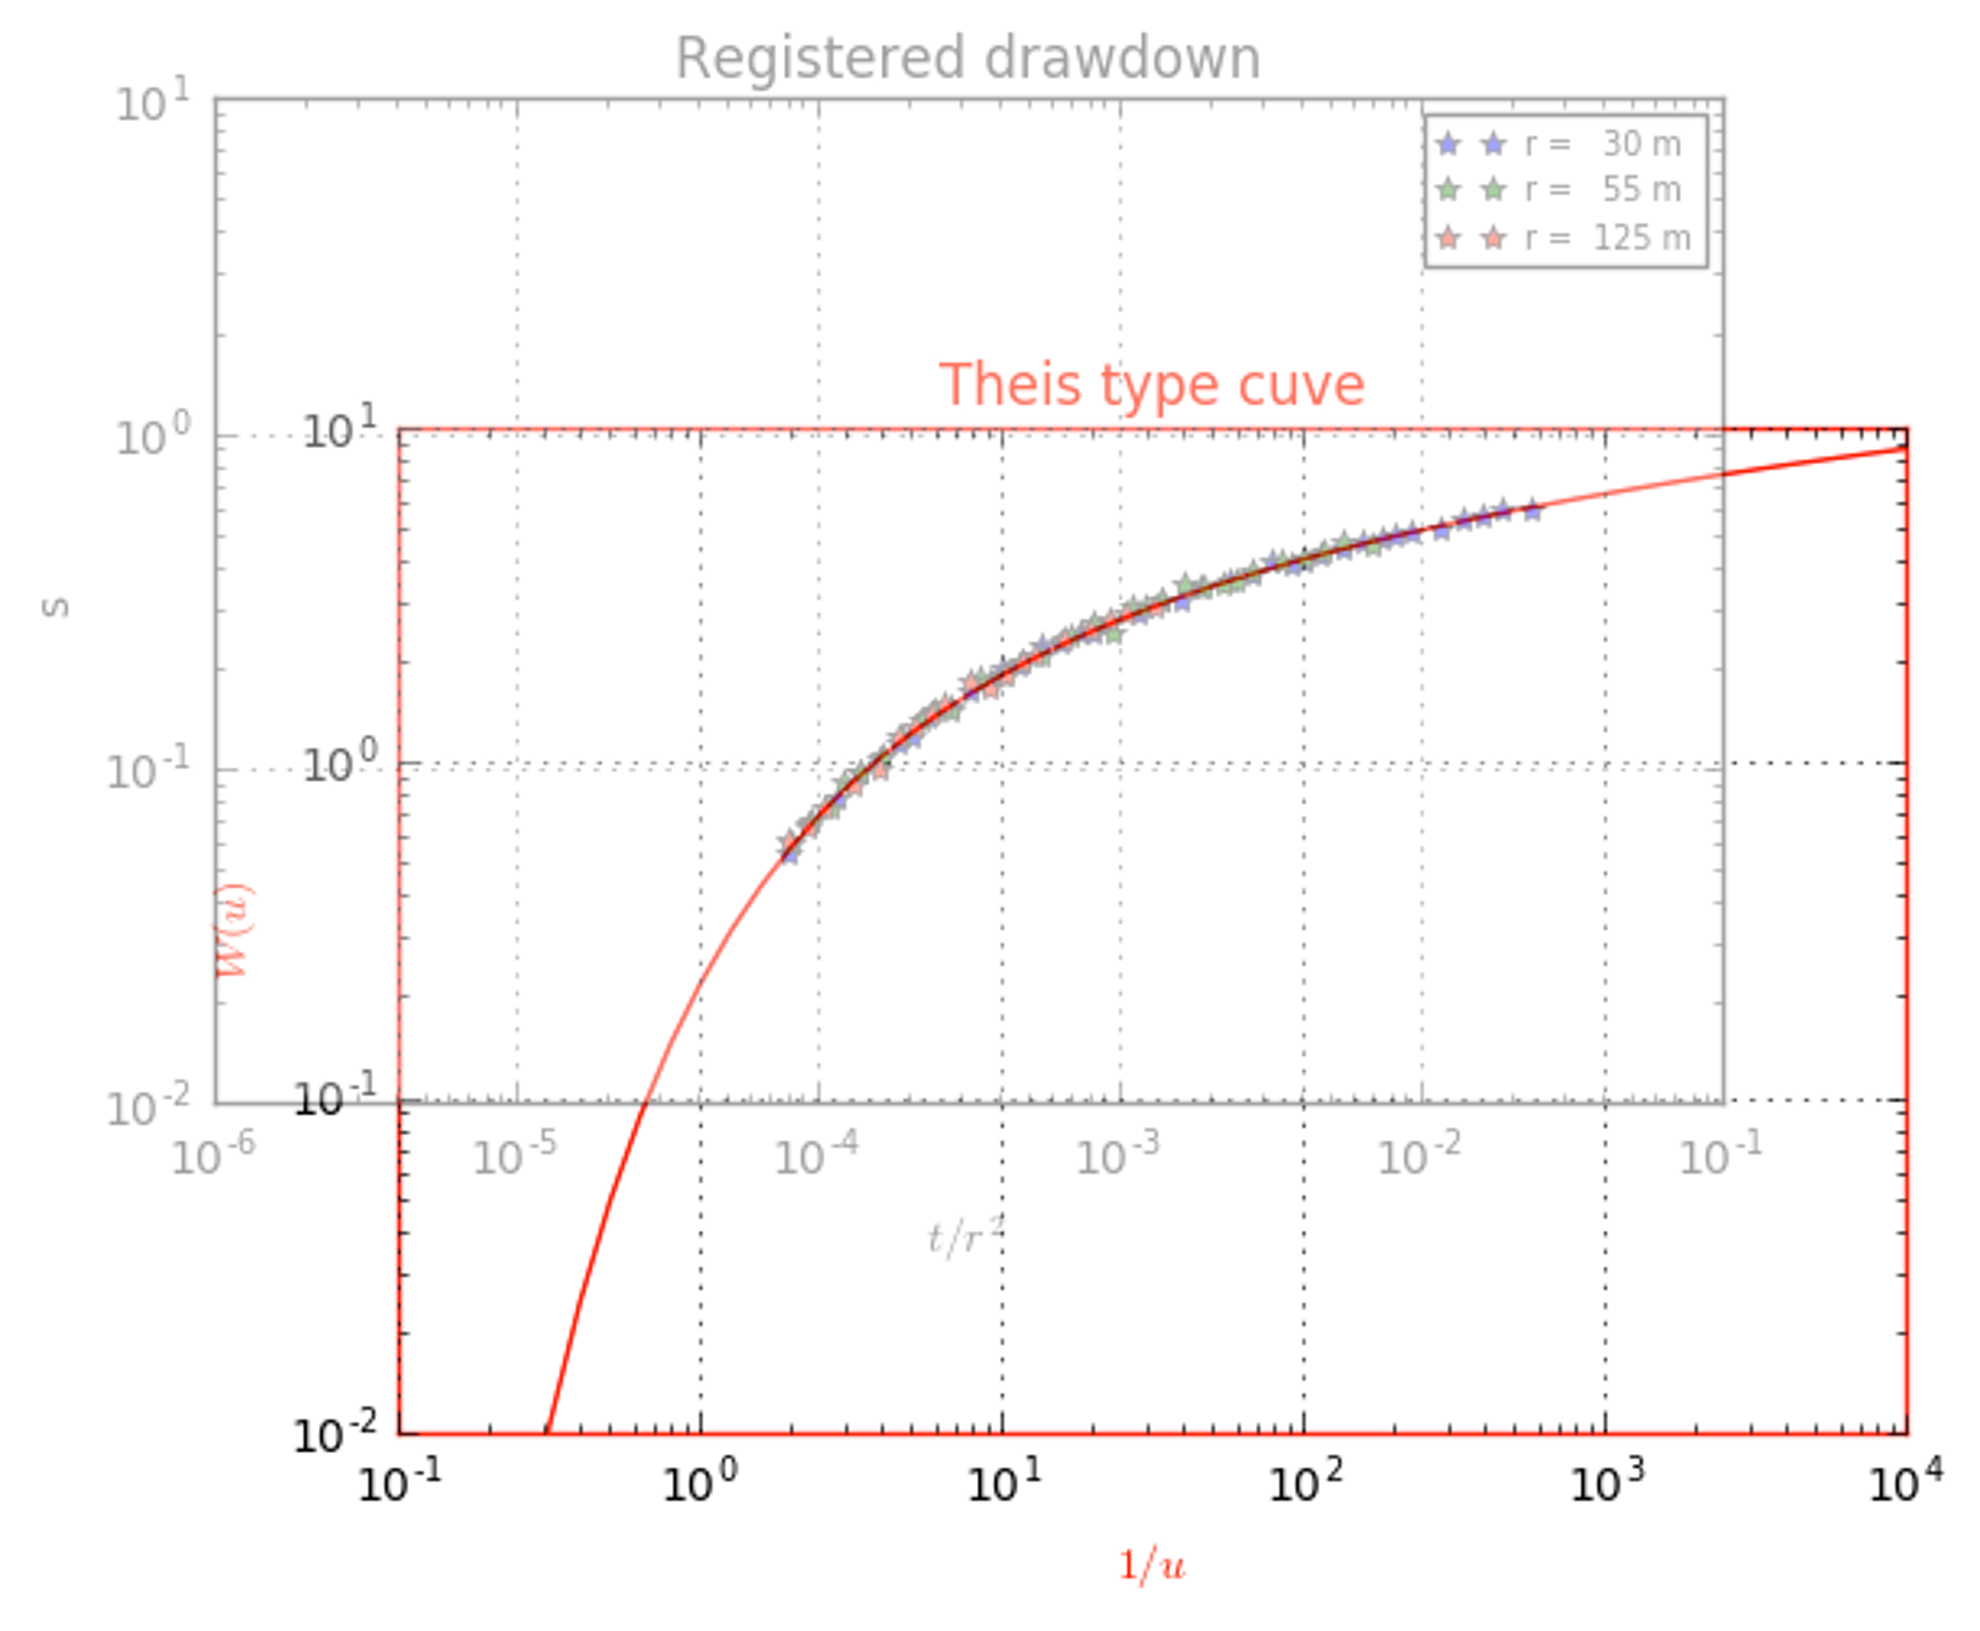
\includegraphics[width=1\textwidth]{pictures/2017_1}
\par\end{centering}
\caption{Measured drawdown curve matched with Theis type curve.}

\end{figure}


\subsection{Question 3}

Imagine the sea tide acting on a shore that has a confined aquifer
inland with a constant \emph{$kD$} and \emph{$S$} in good vertical
contact with the sea. The tide waves, which are characterized by \emph{$A$}
and $\omega$, therefore, penetrate the aquifer; they are mathematically
described by:

\[
s_{x,t}=A\,e^{-ax}\sin\left(\omega t-ax\right)
\]

\begin{enumerate}
\item As can be seen, this equation describes two simultaneous phenomena.
Which are these two phenomena? 
\end{enumerate}
The factor \emph{$a$} in the equation was derived to be

\[
a=\sqrt{\frac{\omega S}{2kD}}
\]

\begin{enumerate}
\item What are the parameters with their dimensions? 
\item A tidal wave has a frequency $\omega$ of two cycles per day of 24
hours, or a cycle time $T$ of 12 hours. Large wind waves, however,
have a cycle time of only about 12 seconds. How far does the influence
of these wind waves penetrate into the aquifer compared to the influence
of the tide waves? Give their ratio and sketch the envelope of both
to show this difference (the sketch does not have to be on scale). 
\end{enumerate}

\section{Closed book reexam (1h), 2016}

\subsection{Question 1}
\begin{enumerate}
\item Explain what barometer efficiency ($BE$) is and how it physically
works.
\item Explain in words what the characteristic (half) time of a groundwater
system is. What does is say about the behavior of the system?
\item For which of the parameters $L$ (system width), $kD$ (transmissivity)
and $S_{y}$ (specific yield) would an increase make the characteristic
system time smaller?
\item Explain why in hydrological logic you think that this is the case.
\item If you see a close-up of two grains held together by a small amount
of water at their point of contact. What then is the pressure in that
water? Explain why that is so.
\end{enumerate}

\subsection{Question 2}

Consider an aquifer in direct contact with the ocean. The tide of
the ocean has an amplitude $A=1.0\,\mathrm{m}$ and the cycle time
is $T=0.5\,\mathrm{d}$ (one full tide in 12h). The aquifer is confined.
It consists of two parts. The first part reaches from the ocean to
500 m inland, the second part is present at more than 500 m from the
ocean. The first part of the aquifer has the following properties:
transmissivity $kD=900\,\mathrm{m^{2}/d}$ and storage coefficient
$S=0.002$. The second part of the aquifer has the following properties:
$kD=1800\,\mathrm{m^{2}/d}$ and storage coefficient $S=0.001$. Because
we consider the fluctuation of the head to be superposed on the mean
head, we are only interested in the head $s$ relative to the mean
head at every location, that is, in $s\left(x,t\right)=h\left(x,t\right)-h\left(x\right)$.
This head fluctuation, $s,$ obeys following expression:

\[
s=A\,e^{-ax}\cos\left(\omega t-ax\right)\mbox{, where }a=\sqrt{\frac{\omega S}{2kD}}\mbox{ and }\omega=\frac{2\pi}{T}
\]

Notice that the storage coefficient is capital $S$ and the head relative
to the mean head is lowercase $s$.
\begin{enumerate}
\item Explain the parameters in the expression and given their dimension
\item What is the amplitude of the groundwater head fluctuation, that is,
the amplitude of $s$, in the aquifer at 500 m and at 1000 m from
the ocean?
\item What is the delay of the head wave at 500 m and 1000 m relative to
the ocean tide? Hint: compute the velocity of the tidal wave in the
aquifer and then the time until the peak of the wave starting at the
ocean reaches $x=500\,\mathrm{m}$ and $x=1000\,\mathrm{m}$.
\end{enumerate}

\subsection{Question 3}

Consider a well in an infinite water table (phreatic) aquifer. Drawdowns
are considered small compared to the thickness of the aquifer, so
that $kD=900\,\mathrm{m^{2}d}$ may be considered constant. The specific
yield, $S_{y}=0.15$, is also constant. As there are no boundary conditions,
the drawdown by the well follows the Theis equation. An approximation
of which is

\[
s\approx\frac{Q}{4\pi kD}\frac{2.3Q}{4\pi kD}\log\left(\frac{2.25kDt}{r^{2}S}\right)
\]

\begin{enumerate}
\item Derive a mathematical expression for the so-called radius of influence,
that is, the distance beyond which the drawdown can be neglected at
a given time $t$ after the well was first switched on.
\item As you can see, the drawdown is a logarithmic function in time. Derive
a mathematical expression of the increase of the drawdown per log
cycle, that is, between for instance $t=6\,\mathrm{d}$ and $t=60\,\mathrm{d}$,
or $t=2\,\mathrm{d}$ and $t=20\,\mathrm{d}$.
\item Assume the well has been continuously pumping for time $t=t$, after
which the extraction was stopped. What is the drawdown at distance
$r_{0}$ at time is $t=t_{1}+\Delta t$ , where $\Delta t$ is any
time passed since $t_{1}$.
\end{enumerate}

\section{Closed-book exam (1h), Feb 1, 2016}

\subsection{Question 1: (16 points)}
\begin{enumerate}
\item Explain loading efficiency, $LE$.
\item Explain the barometer efficiency, $BE$.
\item What is the difference registered by a pressure gauge in a confined
aquifer measuring absolute pressure, given on the one hand a uniform
mass placed at ground surface of weight $\Delta p$ N/m\textsuperscript{2}
and on the other hand a barometer increase of the same value of $\Delta p$
N/m\textsuperscript{2}? 
\item What is the origin of delayed yield? 
\item In which case does the influence of tide reach further inland into
an aquifer? 
\begin{enumerate}
\item The case with the higher or with the lower frequency? 
\item The case with the larger or the smaller transmissivity \emph{kD}? 
\item The case with the larger or with the smaller storage coefficient \emph{S}? 
\end{enumerate}
\item What is the difference between the situations with the wells that
were studied by Theis and by Hantush? 
\item Does the Theis case have a final equilibrium drawdown? Explain your
answer?
\item Does the Hantush case have a final, steady-state drawdown? Explain
your answer?
\end{enumerate}

\subsection{Question 2: (14 points)}
\begin{enumerate}
\item Explain what is the radius of influence of an extraction well in an
aquifer of constant transmissivity and storage coefficient? 
\item The simplified Theis solution is as follows: \\
\[
s\left(r,t\right)\approx\frac{Q}{4\pi kD}\ln\left(\frac{2.25kDt}{r^{2}S}\right)
\]
\end{enumerate}
\begin{quote}
From it derive an expression of the radius of influence. 
\end{quote}
\begin{enumerate}
\item Also show what is the drawdown difference per log cycle of time, that
is, between time is \emph{t} and time is 10\emph{t}. 
\item Consider a well in a water table aquifer at 300 m from an impervious
wall that reaches to the bottom of the aquifer. The aquifer has $kD=600\,\mathrm{m^{2}d}$
and the specific yield of $S_{y}=0.2$. The pumping rate is $Q=1200\,\mathrm{m^{3}/d}$.
Assume that the approximation of the Theis equation that is given
in this question is applicable. Compute the head change of the groundwater
at the wall closest to the well. 
\end{enumerate}

\section{Closed-book exam (1h), Feb 2015}

\subsection{Question 1}
\begin{enumerate}
\item What types of storage or storage coefficients are associated with
transient groundwater flow? And explain short how they physically
work. 
\item Explain the relation between capillary rise and pore diameter 
\item Explain the general shape of the moisture curve in the unsaturated
zone. Describe where the water comes from when the water table is
lowered. 
\item Explain the difference between the loading efficiency (LE) and the
barometer efficiency (BE)? 
\item When you see animal holes in the field, like rabbit, rat and worm
holes, how much do you think these holes may contribute to the infiltration
of rainwater during and after showers, to what extent are the animals
living in those holes affected by heavy rains, and , finally, what
would it take to swim them out of their holes? Explain your answer
from your insight in how water in the subsurface behaves. 
\end{enumerate}

\subsection{Question 2}

Consider a confined aquifer in direct contact with the ocean in which
the head fluctuates along with the tide of the ocean. The daily solar
tide, with cycle time $T=12\,\mathrm{h}$ or, equivalently, $T=0.5\,\mathrm{d}$,
has amplitude $A=2.5\,\mathrm{m}$ and the 4 weekly moon tide, with
cycle time $T=1/28\,\mathrm{d}$, has amplitude or $A=1\,\mathrm{m}$.
The groundwater head in the aquifer relative to the mean value at
time \emph{$t$} and distance \emph{$x$} from the ocean obeys to
the following expression:

\[
s=Ae^{-ax}\cos\left(\omega t-ax\right)\mbox{, where }a=\sqrt{\frac{\omega S}{2kD}}
\]

If \emph{$T$} is the time required for a complete cycle, then the
angular velocity $\omega=2\pi/T$.

Further, \emph{$kD=900\,\mathrm{m^{2}/d}$} and \emph{$S=0.001$}.
\begin{enumerate}
\item Explain the parameters in the expression and give their dimension. 
\item What is the amplitude of the groundwater fluctuation due to both tides
individually at 500 and 2000 m from the coast? So the twice-a-day
tide amplitude at 500 m and at 2000 m and the 28-day tide amplitude
at 500 m and 2000 m? 
\item How much are the waves of both tides delayed at 500 m from the coast? 
\item Over what distance does the maximum tide-induced amplitude in the
groundwater declines by a factor of two in both cases? 
\end{enumerate}

\subsection{Question 3}

A groundwater table rise after it was agitated by a sudden recharge
\emph{N} {[}m{]} will decay over the thereafter. For a system of bounded
by two parallel water courses at \emph{L} mutual distance, this decline
after some time can be approximated by the following expression:

\[
s=A\frac{4}{\pi}\cos\left(\pi\frac{x}{L}\right)\exp\left(-\left(\frac{\pi}{L}\right)^{2}\frac{kD}{S_{y}}t\right)
\]

\begin{enumerate}
\item Describe the parameters and given their dimension. 
\item Give an expression for the sudden rise \emph{A} caused by a sudden
recharge amount equal to N {[}m{]}: 
\item Describe in a few words what this expression is and does, so what
does its graph look like and how does it behave over time. 
\item Give an expression of what can be called characteristic time of this
system. 
\item Derive an expression of the half time of this system. 
\item Derive an expression for the discharge of this system. 
\end{enumerate}

\subsection{Question 4}

A 300 m deep well in Jordan with borehole radius \emph{$r=0.25\,\mathrm{m}$}
was drilled in a limestone aquifer to serve a refugee camp. The well
was recently test pumped during one day at a rate of \emph{$Q=60\,\mathrm{m^{3}/h}$}.
The head at 0, 0.01, 0.1 and 1 d after the start of the pump was 100,
135, 147 and 159 m below ground surface respectively. The pump is
installed at 200 m below ground surface.

Further assume:

The estimated specific yield of this aquifer is 0.01.

The unknown transmissivity is constant.

You may use the simplified expression of transient drawdown in an
infinite aquifer

\[
s\approx\frac{Q}{4\pi kD}\ln\left(\frac{2.25kDt}{r^{2}S}\right)
\]

\begin{enumerate}
\item Estimate the transmissivity of this aquifer. 
\item How much will be the drawdown after 3 years (1000 d)? Is the pump
at 200 m below ground surface (i.e. 100 m below the initial water
table) still deep enough to pump the water up? 
\item Another well of equal size, depth and flow rate is planned at a second
location in the camp at 2 km distance. How much will be the drawdown
in each well after 3 years (1000 days) in this case? Assume that both
wells pump for the same period. How deep should the pumps be installed
to allow pumping both wells at he given rate for 3 years? 
\end{enumerate}

\section{Closed-book reexam (1h), March 2015}

\subsection{Question 1}
\begin{enumerate}
\item Explain what barometer efficiency (BE) is and how it physically works? 
\item When you see animal holes in the field, like rabbit, rat and worm
holes, how much do you think these holes may contribute to the infiltration
of rainwater during and after showers, to what extent are the animals
living in those holes affected by heavy rains, and , finally, what
would it take to swim them out of their holes? Explain your answer
from your insight in how water in the subsurface behaves. 
\end{enumerate}

\subsection{Question 2}

Consider an aquifer in direct contact with the ocean. The tide of
the ocean has an amplitude $A=1\,\mathrm{m}$m and cycle time is \emph{T}
= 0.5 d (one full tide in 12h).

The aquifer is confined. It consists of two parts. The first part
reaches from the ocean to 500 m in land, the second part is present
at more than 500 m from the ocean.

The first part of the aquifer has the following properties: transmissivity
$kD=900\,\mathrm{m^{2}/d}$ and storage coefficient $S=0.002$.

The second part of the aquifer has the following properties, $kD=1800\,\mathrm{m^{2}/d}$
m\textsuperscript{2}/d and storage coefficient $S=0.001$.

Because we consider the fluctuation of the head to be superposed on
the mean head, we are only interested in the head, $s$, relative
to the mean head at every location, that is $s\left(x,t\right)=h\left(x,t\right)-h\left(x\right)$.
This head fluctuation, $s$, obeys following expression:

\[
s=A\,e^{-ax}\cos\left(\omega t-ax\right)\mbox{, where }a=\sqrt{\frac{\omega S}{2kD}}\mbox{ and }\omega=\frac{2\pi}{T}
\]

Notice that the storage coefficient is capital $S$ and the head relative
to the mean head is lower case $s$.
\begin{enumerate}
\item Explain the parameters in the expression and give their dimension. 
\item What is the amplitude of the groundwater head fluctuation, that is,
the amplitude of $s$, in the aquifer at 500 m and at 1000 m from
the ocean? 
\item What is the delay of the head wave at 500 and 1000 m relative to the
ocean tide? Hint: compute the velocity of the tidal wave in the aquifer
and then the time until the peak of the wave starting at the ocean
reaches $x=500\,\mathrm{m}$ and $x=1000\,\mathrm{m}$? 
\end{enumerate}

\subsection{Question 3}

Consider a well in an infinite water-table (phreatic) aquifer. Drawdowns
are considered small compared to the thickness of the aquifer, so
that $kD=900\,\mathrm{m^{2}/d}$ may be considered constant. The specific
yield, $S_{y}=0.15$, is also constant. As there are no boundary conditions,
the drawdown by the well follows the Theis equation. An approximation
of which is

\[
s\approx\frac{2.3Q}{4\pi kD}\log\left(\frac{2.25kDt}{r^{2}S}\right)
\]

\begin{enumerate}
\item Derive a mathematical expression for the so-called radius of influence,
that is, the distance beyond which the drawdown can be neglected at
a given time $t$ after the well was first switched on. 
\item As you can see the drawdown is logarithmic in time. Derive a mathematical
expression for the increase of the drawdown per log cycle, that is
between for instance \emph{$t=6\,\mathrm{d}$} and \emph{$t=60\,\mathrm{d}$}
days, or \emph{$t=2\,\mathrm{d}$} days and \emph{$t=20\,\mathrm{d}$}. 
\item Assume the well has been continuously pumping for time $t=t_{1}$,
after which the extraction was stopped. What is the drawdown at distance
$r_{0}$ at time $t=t_{1}+\Delta t$ , where $\Delta t$ is any time
passed since $t_{1}$. 
\end{enumerate}

\section{Closed book exam, Feb 2014}

\subsection{Question 1}
\begin{enumerate}
\item What types of storage or storage coefficients are associated with
transient groundwater flow?
\item Explain how these types of storage physically work. 
\item Explain the relation between capillary fringe and air entry pressure. 
\item Explain the difference between the loading efficiency (LE) and the
barometer efficiency (BE)? 
\item Why does the specific yield of unconfined aquifers with a shallow
groundwater table depend on the depth of the water table? 
\item What is halftime when considering decay of a water mound between rivers?
How would you describe it? 
\item Assume the well has been continuously pumping for time $t=t_{1}$,
after which the extraction was stopped. What is the drawdown at distance
$r_{0}$ at time $t=t_{1}+\Delta t$ , where $\Delta t$ is any time
passed since $t_{1}$. 
\end{enumerate}

\subsection{Question 2}

Consider a confined aquifer in direct contact with the ocean in which
the head fluctuates along with the tide of the ocean. The tide has
an amplitude of $a=2.5\,\mathrm{m}$. The groundwater head in the
aquifer at time \emph{t} and distance \emph{x} from the ocean obeys
to the following expression:

\[
s=a\,e^{-ax}\cos\left(\omega t-ax\right)\mbox{, where }a=\sqrt{\frac{\omega S}{2kD}}
\]

The frequency $f$ of the tide is one complete cycle per 24 hours,
i.e. $f=1/d$, with, of course, $\omega=2\pi f$.

We don't know the value of \emph{$kD$} and $S$, but we have measured
the amplitude of the groundwater head fluctuation at . This amplitude
is 25 cm, one tenth of that of the ocean.
\begin{enumerate}
\item Explain the parameters in the expression and give their dimension. 
\item Give an expression for the amplitude at distance \emph{x} from the
ocean. 
\item With the given information, compute parameter \emph{a}, and the diffusivity
of the aquifer, i.e. the ratio $kD/S$. 
\item Give an expression for the velocity of the wave of the groundwater-head
in the subsurface? How much is this velocity? 
\end{enumerate}

\subsection{Question 3}

Consider an unconfined aquifer with conductivity $k=10\,\mathrm{m/d}$,
a specific yield of $S_{y}=0.1$ and an initial thickness . A well
is located in this aquifer on each of the four corners of a square
with sides of $L=200\,\mathrm{m}$. The wells start pumping at $t=0$.
They pump with a rate of $Q=120\,\mathrm{m^{3}/d}$ for 1d, after
which they stop.

The drawdown according to Theis is

\[
s=\frac{Q}{4\pi kD}\mathrm{W}\left(u\right)\mbox{, where }u=\frac{r^{2}S}{4kDt}
\]

The Theis well function is graphically given in Figure 1 below.
\begin{enumerate}
\item Compute the drawdown in the center of the square after $t=2\,\mathrm{d}$.
You may neglect the change of the transmissivity caused by the change
of the water depth in the aquifer. 
\end{enumerate}

\subsection{Question 4}

Given that the well function can be computed by the following infinite
series

\[
\mathrm{W}\left(u\right)=-\gamma-\ln u+u-\frac{u^{2}}{2\times2!}+\frac{u^{3}}{3\times3!}-\frac{u^{4}}{4\times4!}+\cdots
\]

with $\gamma=0.577216\cdots$ and $u=r^{2}S/\left(4kDt\right)$
\begin{enumerate}
\item What would be a good approximation of the drawdown for small values
of $u$? (Assume for instance that \emph{u}<0.01). Notice for mathematical
convenience, that $\gamma=\ln\left(e^{\gamma}\right)$. 
\item How could you define the radius of influence of the drawdown? Use
the formula for the drawdown from the previous question together with
the approximation from the previous question. 
\end{enumerate}
\begin{figure}
\begin{centering}
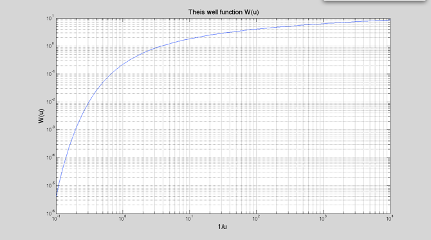
\includegraphics[width=0.8\textwidth]{pictures/2014_1}
\par\end{centering}
\caption{Theis well function type curve, ie, $\mathrm{W}\left(u\right)$ versus
$1/u$.}

\end{figure}


\section{Closed-book exam (1h), Feb 3, 2011}

\subsection{Question 1: Pressure in confined aquifer}

Question 1: Pressure in confined aquifer

A water level in a piezometer in a confined aquifer is affected if
the weight on a ground surface is suddenly changed. Compare two situations
a) Sudden change by a load placed on the ground, such as sand or flooding
by water and b) Sudden increase of the barometric pressure.

Case a: --- a load is placed on ground surface
\begin{enumerate}
\item How does the water pressure change in the piezometer? (Up? Down? Not?) 
\item How does the head change in the piezometer? (Up? Down? Not?) 
\end{enumerate}
Case b: --- barometer pressure increased
\begin{enumerate}
\item How does the water pressure change in the piezometer? (Up? Down? Not? 
\item How does the head change in the piezometer? (Up? Down? Not?) 
\end{enumerate}
General:
\begin{enumerate}
\item If there is a difference between the two cases, then why is that? 
\end{enumerate}

\subsection{Question 2}

The groundwater head variation in a confined aquifer due to a tidal
wave at x=0 can be expressed mathematically as follows:

\[
s\left(x,t\right)=\phi\left(x,t\right)-\phi_{0}+A\,\exp\left(-ax\right)\sin\left(\omega t-ax\right)\mbox{, in which }a=\sqrt{\frac{\omega S}{2kD}}
\]

and $\omega=\frac{2\pi}{T}$ with $T$ the period of the wave.
\begin{enumerate}
\item What is the amplitude of the wave at distance $x$? 
\item What is the velocity of the wave? 
\item If the wave would be just observable in a piezometer at $x=1000\,\mathrm{m}$
from the coast, then at what distance would the wave be just observable
on another spot along the coast where the storage coefficient is be
100 times greater than at the current spot and the transmissivity
is the same? 
\item A tidal wave occurring daily is just observable in the aquifer at
a distance of $x=500\,\mathrm{m}$ from shore, where $x=0$. At what
distance from the shore will a 14-day wave be just observable occurring
due to the monthly moon cycle? Assume the same amplitude for both
waves. 
\end{enumerate}

\subsection{Question 3}

In class we discussed the somewhat complicated solution by series
expansion of the evolution of the head after a sudden rain shower
of $P$ {[}m{]} in a strip of land of width $L$ {[}m{]} between parallel
fixed-head boundaries with water level $\phi_{0}$ {[}m{]}. We have
seen that after some time $t$ {[}d{]}, only the first term matters,
which is

\[
s\left(x,t\right)=\phi\left(x,t\right)-\phi_{0}=\frac{P}{S_{y}}\frac{4}{\pi}\cos\left(\pi\frac{x}{L}\right)\exp\left(-\pi^{2}\frac{kD}{L^{2}S_{y}}t\right)
\]

Whenever possible express your answers mathematically:
\begin{enumerate}
\item What is the shape of the head? 
\item What is the maximum head, take $\phi_{0}=0$? 
\item What would you consider the characteristic time of this system? 
\item What would be the half-time of this groundwater system? 
\end{enumerate}

\subsection{Question 4: wells}

The solution by Theis is given by

\[
s\left(r,t\right)=\phi_{0}-\phi\left(r,t\right)=\frac{Q_{0}}{4\pi kD}\mathrm{W}\left(u\right)\mbox{, where }u=\frac{r^{2}S}{4kDt}
\]

\begin{enumerate}
\item What flow conditions are described by Theis' well solution? 
\item What are its parameters and what are their dimensions? 
\end{enumerate}
As you know, the function W($u$) is the exponential integral, which
may be written as a series expansion :

\[
\mathrm{W}\left(u\right)=-0.577316-\ln u+u-\frac{u^{2}}{2\times2!}-\frac{u^{3}}{3\times3!}+\frac{u^{4}}{4\times4!}\cdots
\]

\begin{enumerate}
\item How can you mathematically approximate the Theis' solution for very
small values of $u$ given that $-0.577216\approx\ln\left(0.5615\right)$?
\item With this approximation, mathematically give the difference between
the drawdown obtained at time t and the drawdown at time 10t in a
piezometer at some arbitrary distance r from the well. 
\end{enumerate}
You may use the fact that $\ln10\approx2.3$.

Also give the difference between the drawdown in a piezometer at distance
r from the well and in a piezometer at distance 10r from the well,
both at the same time.

\section{Closed-book exam (1h), Feb 2010}

\subsection{Question 1}
\begin{enumerate}
\item What is liquefaction? 
\item What is the difference between specific yield and elastic storage? 
\item How does the specific yield change if an already shallow water table
rises? 
\item Why does this happen (make a sketch and explain) 
\item Which of the two materials, gravel and fine sand, has the highest
specific yield and why (assume both have the same porosity)? 
\end{enumerate}

\subsection{Question 2}

The head in an aquifer connected to the ocean fluctuates due to tide.
This fluctuation is given by the following formula, in which \emph{s}
expresses the head variation caused by the tide as a function of time
\emph{t} and the inland distance from the shore \emph{x}:
\begin{quote}
\[
s\left(x,t\right)=A\,\exp\left(-ax\right)\sin\left(\omega t-ax\right)\mbox{, with }a=\sqrt{\frac{\omega S}{2kD}}
\]
\end{quote}
\begin{enumerate}
\item What is the expression for the maximum head fluctuation as a function
of \emph{x}? 
\item Sketch the head change \emph{s} as a function of \emph{x} at time
\emph{t}=0 and sketch also the envelope (maximum and minimum value
of \emph{s} as a function of \emph{x}) 
\item Which parameters increase the inland penetration of the tide and which
parameters decrease this inland penetration? 
\end{enumerate}

\subsection{Question 3}

Consider an extraction canal in direct contact with an aquifer of
infinite extent. The aquifer has transmissivity $kD=400\,\mathrm{m^{2}/d}$
and specific yield $S_{y}=0.1$. As long as $t<0$, the head in the
aquifer is everywhere 0 m (we take the initial water level as our
reference level).

At time $t=0\,\mathrm{d}$, the water level in the canal suddenly
changes to 2 m. Then, at time $t=2~\mathrm{d}$, the water level in
the canal suddenly changes back to its original value of 0 m and remains
constant afterwards.

The head change and the head-change gradient are:

\[
s=s_{0}\mathrm{erfc}\left(\sqrt{\frac{x^{2}S}{4kDt}}\right)\mbox{ and }\frac{\partial s}{\partial x}=-s_{0}\sqrt{\frac{S}{\pi kDt}}\exp\left(-\frac{x^{2}S}{4kDt}\right)
\]

To obtain values for the \textbf{$\mathrm{erfc}$ }function, use the
graph below.

Answer the following two questions.
\begin{enumerate}
\item Compute the head at $x=100\,\mathrm{m}$ at $t=3\,\mathrm{d}$. Show
the formula you use and include the dimension in your answer! 
\item Compute the discharge at $x=0$ at $t=3\,\mathrm{d}$. Show the formula
you use and include the dimension in your answer?
\end{enumerate}
\begin{figure}
\begin{centering}
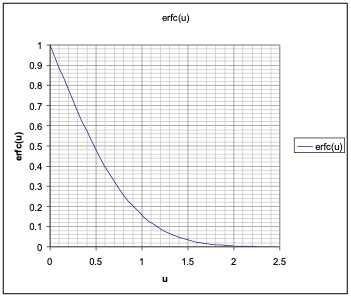
\includegraphics[width=0.7\textwidth]{pictures/2010_1}
\par\end{centering}
\caption{Function $\mathrm{erfc}\left(u\right)$}

\end{figure}


\subsection{Question 4}

Consider a well in a system of infinite extent which starts extracting
at time \emph{t}=0. We know that Theis' formula applies:

\[
s\left(r,t\right)=\frac{Q}{4\pi kD}\mathrm{W}\left(u\right)\mbox{, where }u=\frac{r^{2}S}{4kDt}
\]

We also know that for small values of \emph{u}, the well function,
W($u$), can be approximated by a straight line on log-t scale, which
is given by:

\[
\mathrm{W}\left(u\right)\approx2.3\log\left(\frac{0.5625}{u}\right)=2.3\log\left(\frac{2.25kDt}{r^{2}S}\right)
\]

Consider a pumping test on this well, starting the constant extraction
$Q=800\,\mathrm{m^{3}/d}$ at $t=0$. The drawdown is measured over
a number of days at an observation well at 25 m distance. The measured
drawdowns are shown in the figure below, which clearly reveals the
straight portion of the drawdown that we expect from the expression
above for large-enough values of time.
\begin{enumerate}
\item Using the straight line through the measured data, compute the transmissivity
\emph{$kD$} and the storage coefficient \emph{$S$} of this aquifer.
\end{enumerate}
\begin{figure}
\begin{centering}
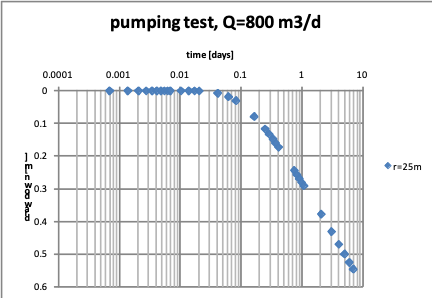
\includegraphics[width=0.8\textwidth]{pictures/2010_2}
\par\end{centering}
\caption{Measured drawdown during pumping test.}

\end{figure}


\section{Closed-book exam (3h), Feb 2009}

\subsection{Question 1}
\begin{enumerate}
\item What is the difference between specific yield and elastic storage? 
\item How does the specific yield change if an already shallow water table
rises further and becomes even shallower? 
\item Why does this happen (make a sketch and explain) 
\item Which of the two materials, gravel and fine sand, has the highest
specific yield and why (assume both have the same porosity)? 
\end{enumerate}

\subsection{Question 2}
\begin{enumerate}
\item What do we mean by Loading Efficiency ($LE$) and what do we mean
by Barometric Efficiency ($BE$)? 
\item What is the difference in terms of head change if we compare a loading
on land surface with an equal increase of the barometer pressure?
And why? 
\end{enumerate}

\subsection{Question 3}

Tidal flow in a confined aquifer may be described mathematically by

\[
s=A\,e^{-ax}\sin\left(\omega t-ax\right)\mbox{, where }a=\sqrt{\frac{\omega S}{2kD}}
\]

\begin{enumerate}
\item What are the different quantities in these expressions and what are
their dimensions?
\item By what expression is the envelope given (the envelope describes the
maximum amplitude as a function of $x$?) 
\item How does the envelope change if the frequency of the tide would double? 
\item How will the envelope change if the transmissivity would be two times
less and the storage coefficient 100 times less? 
\end{enumerate}

\subsection{Question 4}

The picture below shows a strip of land of width \emph{L} bounded
by two canals. Both the strip and the canals run perpendicular to
the paper (so the picture is a cross section). Suddenly the water
level in the left canal is raised by \emph{A} m as is indicated in
the figure. This causes the head to change in the strip. At the right
hand side the water level is unchanged. There exists an expression,
which mathematically describes the effect of a sudden level rise in
a strip that is unbounded on one side. We want to use this expression
to compute the head in the strip. We can do this by means of mirror
canals.

\begin{figure}
\begin{centering}
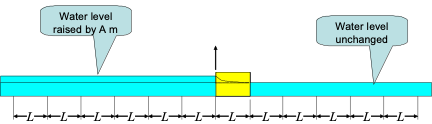
\includegraphics[width=1\textwidth]{pictures/2009_1}
\par\end{centering}
\caption{Strip of land of width \emph{L} bounded by open water. The water level
at the left hand side was suddenly raised by \emph{A} m. This causes
the head in the aquifer of the strip to change dynamically.}

\end{figure}

\begin{enumerate}
\item Irrespective of what the mathematical looks like, where would you
put the mirror canals and which are positive and which are negative?
Just draw an arrow respectively up or down (see figure) at the locations
where you would put the mirror canal.
\end{enumerate}


\subsection{Question 4}

The characteristic dynamics of a groundwater systems (i.e., the time
it takes for the head of a groundwater system to reach equilibrium)
is related to the argument of transient groundwater flow solutions,
This argument is $\sqrt{\frac{x^{2}S}{4kDt}}$ in solutions for one-dimensional
flow and $\frac{r^{2}S}{4kDt}$ for radial flow such as in the well
functions of Theis and Hantush.
\begin{enumerate}
\item Explain how the characteristic dynamics relate to these arguments? 
\item Compare the characteristic dynamics of two systems. System two is
twice as wide as system one and its transmissivity is 3 times as large
and its storage coefficient 100 times as small as that of system one.
How do the dynamics of these two systems relate to each other, that
is: how many times faster or slower is system two compared to system
one in reaching piezometric equilibrium? 
\end{enumerate}

\subsection{Question 5}

Consider a well in a semi-confined aquifer with $kD=900\,\mathrm{m^{2}/d}$,
$S=0.001$ and $c=400\,\mathrm{d}$ that is pumped at a discharge
$Q=2400\,\mathrm{m^{3}/d}$.
\begin{enumerate}
\item How long does it take before the drawdown at 60 m distance from the
well becomes stationary? 
\item What is the final drawdown? 
\end{enumerate}

\subsection{Question 6}

A pumping test has been carried out in a confined aquifer. The drawdown
and the Theis type curves are given in the graphs below. Theses graphs
have been drawn on the same type of double logarithmic paper. The
extraction of the well during the test was 1000 m\textsuperscript{3}/d.
Determine the transmissivity and the storage coefficient of this groundwater
system.

\begin{figure}
\begin{centering}
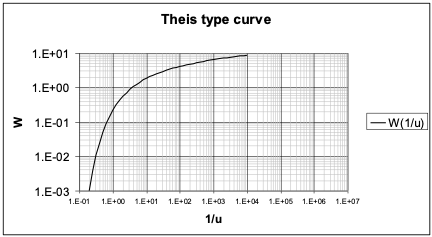
\includegraphics[width=0.8\textwidth]{pictures/2009_3}
\par\end{centering}
\caption{Theis well function Type curve.}

\end{figure}

\begin{figure}
\begin{centering}
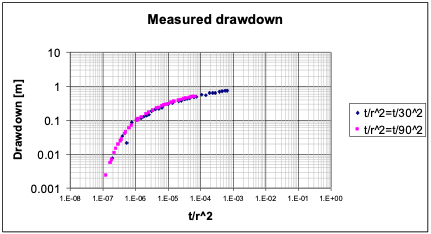
\includegraphics[width=0.8\textwidth]{pictures/2009_4}
\par\end{centering}
\caption{Measured drawdown versus $t/r^{2}.$}

\end{figure}

\begin{figure}

\begin{centering}
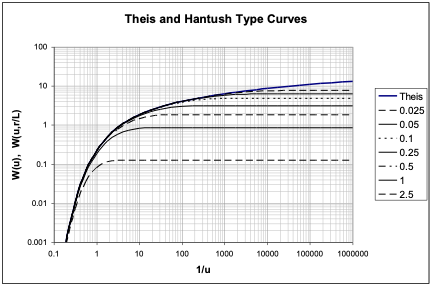
\includegraphics[width=0.8\textwidth]{pictures/2009_5}
\par\end{centering}
\caption{Theis and Hantush well function type curves.}

\end{figure}


\section{Closed-book exam (3h), Feb 2007}

\subsection{Question 1: General}
\begin{enumerate}
\item What is specific yield?
\item How does specific yield depend on the distance of the water table
below ground level? 
\item What happens to the water table in a piezometer in a confined aquifer
when the barometer pressure goes up, why? 
\end{enumerate}

\subsection{Question 2: Diffusion equation}

The diffusion equation for transient flow in one dimension is $D\frac{\partial^{2}s}{\partial x^{2}}=\frac{\partial s}{\partial t}$
\begin{enumerate}
\item What is the dimension of the diffusivity \emph{D}? 
\item What is diffusivity \emph{D} in the case of groundwater flow? 
\item What is diffusivity \emph{D} in the case of heat flow? 
\end{enumerate}

\subsection{Question 3: Fluctuation groundwater}

In the case of a tidal fluctuation in a river in direct contact with
an aquifer having transmissivity the fluctuation of the head may be
described by

\[
s=s_{0}\exp\left(-ax\right)\sin\left(\omega t-ax\right)\mbox{, with }a=\sqrt{\frac{\omega S}{2kD}}
\]

\begin{enumerate}
\item What is \emph{$s$} and what does this function look like? Make a
sketch of \emph{s} as a function of \emph{x}, and show its envelopes.
(The envelope is the curve of the values between which the function
fluctuates, as a function of $x$).
\item In the case of a double-day tide, $\omega=\frac{4\pi}{24}\,\mathrm{h^{-1}}$,
what would be the speed of the wave into the aquifer if $S=0.001$
and $kD=500\,\mathrm{m^{2}/d}$? (Notice the dimensions!) 
\item What happens to this distance in case the transmissivity would be
9 times a big? 
\end{enumerate}

\subsection{Question 4: Flow to an extraction canal}

Consider an extraction canal in direct full contact with an aquifer
with transmissivity $kD=400\,\mathrm{m^{2}/d}$ and specific yield
$S_{y}=0.1$. The water level in the canal suddenly changes by 2 m
downward. The head and gradient are given by:

\[
s=s_{0}\mathrm{erfc}\left(\sqrt{\frac{x^{2}S}{4kDt}}\right)\mbox{ and }\frac{\partial s}{\partial x}=-s_{0}\sqrt{\frac{S}{\pi kDt}}\exp\left(-\frac{x^{2}S}{4kDt}\right)
\]

\begin{enumerate}
\item Compute the discharge into the canal after 1d. Show the formula you
use and include the dimension in your answer! 
\item What is the head change \emph{s} at 100 m from the canal after 1 and
after 2 d? (Use erfc-curve further down). 
\item What is the head change at 100 m from the canal after 2 days if the
head in the river would change back by 2 m at \emph{t}=1d? 
\end{enumerate}

\subsection{Question 4: Well in semi-confined aquifer}

Consider a transient well in a semi0-confined aquifer so that Hantush's
solution is valid, hence,

\[
s=\frac{Q}{4\pi kD}\mathrm{W}\left(u,\frac{r}{\lambda}\right)\mbox{, with }u=\frac{r^{2}S}{4kDt}\mbox{ and }\lambda=\sqrt{kDc}
\]

with $kD=600\,\mathrm{m^{3}/d}$, $c=900\,\mathrm{d}$, $S=0.001$
and pumping at a rate $Q=2400\,\mathrm{m^{3}/d}$.
\begin{enumerate}
\item How long does it take before steady state is reached for a point at
\emph{r}=300 m from the well (why)? Use Hantush type curves (see graphic
at the end of this exam). 
\end{enumerate}

\subsection{Question 6: Drawdown due to a pumping station in an unconfined aquifer}

A well is situated at 100 m from an impermeable infinitely long wall.
The well is pumping at a rate of 2400 m\textsuperscript{3}/d. Even
though the aquifer is unconfined, the transmissivity \emph{$kD$}
may be taken as a constant equal to 600 m\textsuperscript{2}/d, while
the specific yield \emph{$S_{y}$}\textsubscript{} equals 0.2. The
well bore has a radius of $r_{0}=0.25\,\mathrm{m}$.
\begin{enumerate}
\item What is the drawdown at the well bore after 10 days of pumping ? 
\item A well in a confined aquifer of infinite extent, with $kD=1000\,\mathrm{m^{2}/d}$
and $S=0.001$, is pumping at a rate of $Q=24000\,\mathrm{m^{3}/d}$.
How far would the radius of influence of this well after 100 years?
The radius of influence is the radius beyond which the drawdown is
considered negligible. You may exploit the logarithmic approximation
of the Theis well function for large times: 
\end{enumerate}
\[
\mathrm{W}\left(u\right)\approx\ln\left(\frac{0.5625}{u}\right)\mbox{, with }u<0.1\mbox{ and }u=\frac{r^{2}S}{4kDt}
\]

by making it zero.

\begin{figure}
\begin{centering}
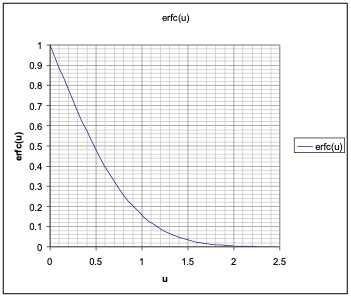
\includegraphics[width=0.8\textwidth]{pictures/2007_1}
\par\end{centering}
\caption{$\mathrm{erfc}\left(u\right)$function.}

\end{figure}

\begin{figure}
\begin{centering}
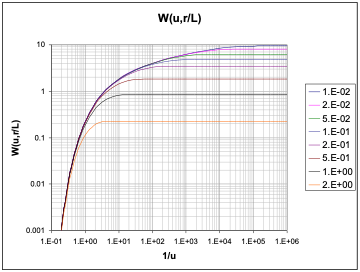
\includegraphics[width=0.8\textwidth]{pictures/2007_2}
\par\end{centering}
\caption{Theis and Hantush type curves. In case this graph is copied in black
and white only, note that the lowest type curve is for the highest
value of \emph{$r/\lambda$.} Note that the $L$ in the title and
left axis of this figure stands for $\lambda=\sqrt{kDc}$ value}

\end{figure}


\section{Closed-book exam (3h), Feb 2006}

\subsection{Question 1: Conceptual}
\begin{enumerate}
\item What types of reversible storage do you know in aquifer systems, explain
how it works 
\item What values may you expect for the respective storage coefficients? 
\item What is barometric efficiency, explain how it works. 
\item When the barometric pressure increases, does the head (water table
in a piezometer) in the confined aquifer rise or fall? 
\item Between what values may the barometric efficiency vary? 
\item What happens in a confined aquifer with the head if a load is suddenly
placed on ground surface, such as a train stopping near a piezometer?
What happens when it leaves? Sketch a graph showing the head versus
time that you would expect in that case. 
\end{enumerate}

\subsection{Question 2: Characteristic time of groundwater basin}

Characteristic time of groundwater basin, the partial differential
equation of which reads

\[
kD\frac{\partial^{2}\phi}{\partial x^{2}}=S\frac{\partial\phi}{\partial t}
\]

\begin{enumerate}
\item What is a characteristic time of a groundwater basin that may be considered
as one-dimensional of characteristic size \emph{L}? (hint: Make partial
differential equation dimensionless by setting $\xi=\frac{x}{L}$,
$\tau=\frac{t}{T}$ and see what $T$ is. 
\item To reach equilibrium, how many times slower is a large basin compared
to a small one with the same transmissivity and storage coefficient? 
\item Compute the characteristic time for the following cases:
\begin{enumerate}
\item Large basin: $kD=500\,\mathrm{m^{2}/s}$ , system width $L=100\,\mathrm{km}$,
storage coefficient $S=0.2$, 
\item Small basin: $kD=100\,\mathrm{m^{2}/d}$, system width $L=100\,\mathrm{m}$
, storage coefficient $S=0.1$. 
\end{enumerate}
\end{enumerate}

\subsection{Question 3: Tides in groundwater}
\begin{quote}
Given: The tidal fluctuation in an aquifer in a point at distance
\emph{x} from the sea due to the water level fluctuation at sea with
amplitude \emph{A} is described by the following formula

\[
s\left(x,t\right)=A\,\exp\left(-ax\right)\sin\left(\omega t-ax\right)
\]

in which the damping factor is as follows $a=\sqrt{\frac{\omega S}{2kD}}$,
where $\omega$ is the angle velocity in radians/time or $\omega=\frac{2\pi}{T}$
where $T$ is the time of a complete wave cycle. 
\end{quote}
Are the following expressions true or false?
\begin{enumerate}
\item The wave in the aquifer has a different frequency than the tide itself.
\item The amplitude of the wave at a given distance from the sea becomes
greater when,
\begin{enumerate}
\item the frequency of the tide is reduced 
\item the storage coefficient is reduced 
\item then the transmissivity is reduced 
\end{enumerate}
\end{enumerate}

\subsection{Question 4: Aquifer with river}

Consider an aquifer of infinite extent bounded by a fully penetrating
river at $x=0$. At $t=0$ the river level suddenly changes by a height
$A$. The change of head $s(x,t)$ in the aquifer equals in this case:

\[
s\left(x,t\right)=A\,\mathrm{erfc}\left(\sqrt{\frac{x^{2}S}{4kDt}}\right)
\]

with $\mathrm{erfc}(u)$ as shown in the picture below

\begin{figure}
\begin{centering}
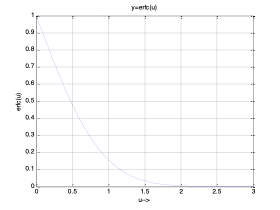
\includegraphics[width=0.8\textwidth]{pictures/2006_1}
\par\end{centering}
\caption{$\mathrm{erfc\left(u\right)}$versus $u$}

\end{figure}

\begin{enumerate}
\item What is the final value of the head change (the value reached after
infinite time, $s\left(x,\infty\right)$? 
\item What value has the argument of $\mathrm{erfc}(\cdots)$, i.e., $\sqrt{\frac{x^{2}S}{4kDt}}$
when the head change is half the final value? 
\item If $kD=400\,\mathrm{m^{2}/d}$, $S=0.1$ and $x=100\,\mathrm{m}$,
after how much time is this the change of head equal to $0.5A$? 
\item What would be the formula if the head change occurred on time \emph{$t_{1}$}\textsubscript{}
instead of time$t=0$? 
\item How could you compute the head change at point \emph{$x$} if the
there was a sudden change of the river level of \emph{$A_{1}$} at
time \emph{$t=t_{1}$} and another of \emph{$A_{2}$}\textsubscript{}
at \emph{$t=t_{2}$}? 
\end{enumerate}

\subsection{Question 5: Well in a confined aquifer}

Consider a well in a confined aquifer starting an extraction of $Q=1200\,\mathrm{m^{3}/d}$
at $t=0$. $kD=1000\,\mathrm{m^{2}/d}$, and $S=0.001$. For this
case the Theis solution applies:

\[
s=\frac{Q}{4\pi kD}\mathrm{W\left(u\right)\mbox{, with }}u=\frac{r^{2}S}{4kDt}
\]

(See the type curve of Theis well function on a separate page).
\begin{enumerate}
\item Compute the head at $r=20\,\mathrm{m}$ after $t=1\,\mathrm{d}$. 
\item The pump is switched off after 1 day. What is the head after 1.1 days
at $r=20\,\mathrm{m}$? 
\end{enumerate}

\subsection{Question 6: Well in a leaky aquifer}

Consider a transient well in a leaky aquifer. $kD=400\,\mathrm{m^{2}/d}$,
$c=400\,\mathrm{d}$, $S=0.001$, so that the groundwater behaves
according to Hantush's transient well formula

\[
s=\frac{Q}{4\pi kD}\mathrm{W}\left(u,\frac{r}{\lambda}\right)\mbox{, with }\lambda=\sqrt{kDc}
\]

\begin{enumerate}
\item How long does it take until the head at $r=40\,\mathrm{m}$ becomes
steady state or virtually steady state? (Hint: look at the type curves
to get u for which this is the case, note). 
\end{enumerate}

\subsection{Question 7: Well in an unconfined aquifer}

Consider a well in an unconfined aquifer for which the Theis-solution
applies (see type curve hereafter. Further given a pumping test with
an extraction of $Q=600\,\mathrm{m^{3}/d}$ during which drawdown
measurements were made (see the graph with the small circles).

Interpret the test (that is: compute \emph{kD} and \emph{S}).

(Hint: if you can't see through the paper make the type curve thicker
using a pen and hold both curves up against a light or in the direction
of a window).

\begin{figure}
\begin{centering}
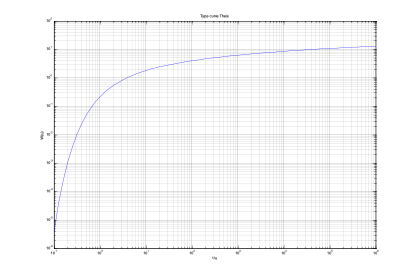
\includegraphics[width=0.8\textwidth]{pictures/2006_2}
\par\end{centering}
\caption{Theis type curve, $\mathrm{W}\left(u\right)$ versus $1/u$}

\end{figure}

\begin{figure}
\begin{centering}
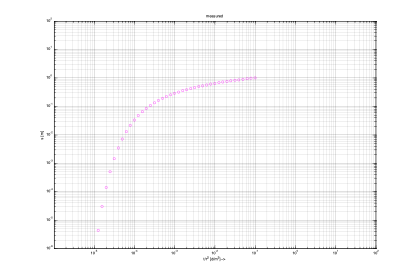
\includegraphics[width=0.8\textwidth]{pictures/2006_3}
\par\end{centering}
\caption{Measured drawdown during pumping test versus \emph{$t/r^{2}$})}

\end{figure}

\begin{figure}
\begin{centering}
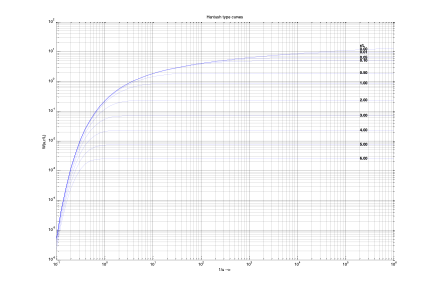
\includegraphics[width=0.8\textwidth]{pictures/2006_4}
\par\end{centering}
\caption{Theis and Hantush type curves combined, i.e., $\mathrm{W}\left(u\right)$
and $\mathrm{W}\left(u,\frac{r}{\lambda}\right)$ vs $1/u$.}

\end{figure}

\end{document}
